\documentclass{article}

% Language setting
% Replace `english' with e.g. `spanish' to change the document language
\usepackage[english]{babel}

% Set page size and margins
% Replace `letterpaper' with`a4paper' for UK/EU standard size
\usepackage[letterpaper,top=2cm,bottom=2cm,left=3cm,right=3cm,marginparwidth=1.75cm]{geometry}

% Useful packages
\usepackage[colorlinks=true, allcolors=blue]{hyperref}
\usepackage{amsmath}
\usepackage{graphicx}
\usepackage{algpseudocode}
\usepackage{algorithm}
\usepackage{amssymb}
\usepackage{xcolor}
\usepackage{tikz}
\usetikzlibrary{automata, positioning, arrows}
\usepackage{amsthm}

\tikzset{
->, % makes the edges directed
>=stealth, % makes the arrow heads bold
node distance=3cm, % specifies the minimum distance between two nodes. Change if necessary.
every state/.style={thick, fill=gray!10}, % sets the properties for each ’state’ node
initial text=$ $, % sets the text that appears on the start arrow
}
\tikzset{
  mydotted/.style={dotted, line width=1pt}
}

\title{ \large Theory of Computation  \\ \LARGE  Pumping Lemma}
\author{Mayank Yadav}
\date{February 12, 2025}

\begin{document}
\maketitle


\section{Introduction}
Pumping Lemma describes an essential characteristic of regular languages. It says that a string with sufficiently long length belonging to a regular language can be divided into three sections, then the string obtained by pumping(or repeating) the middle section also belongs to the same language.

\begin{center}
\fbox{%
    \parbox{0.9\textwidth}{
        Pumping Lemma states that for given a regular language $L$, there exists an integer $p\ge 1$ such that every string $w$ having $\mid w \mid \ge p$ can be expressed as $w=xyz$ and the following conditions hold:\\
        $$\mid y\mid \ge 1$$ 
        $$\mid xy\mid \le p$$
        $$(\forall n\ge 0) (xy^nz\in L) $$
        Mathematically,
        $$
        \forall L \subseteq \Sigma^*, \text{ regular}(L) 
        $$
        $$
        \implies  \exists p \geq 1, \forall w \in L, \mid w\mid  \geq p 
        $$
        $$
        \implies  \exists x, y, z \in \Sigma^*, (w = xyz) \land (\mid y\mid  \geq 1) \land (\mid xy\mid  \leq p) \land (\forall n \geq 0, xy^n z \in L)
        $$
    }
}
\end{center}

We can get intuitions behind this lemma by considering a DFA that accepts a regular language $L$ (as the language is regular we can construct a DFA), let $w$ be a string in $L$ having length at least $p$ say $n$. Let $A$,$B$ and $C$ be some of the states through which $w$ goes through. As $w$ is in the language, it will be accepted by DFA so C is a final state. As each character corresponds to a transition, the number of characters is equal to the number of transitions, hence there are $n$ transitions so $n+1$ states from initial to the final state. As $n\ge p\implies n+1>p$, hence according to pigeonhole principle there is a repetition of one state and say it is $B$. 

We can divide the string $w$ into $x,y,z$; $x$ being the part before reaching $B$, $y$ being the part between two occurrences of $B$ and $z$ being the part after B.

We can now check the conditions given in the lemma, $\mid y\mid\ge 1$ as that is the part that occurs between two repetition of $B$, $\mid xy\mid \le p$ as a repetition occurs in $p+1$ states and third condition holds as $y$ is being handled in the loop, so for example in $xyyz$, the both $y$ get handled by the loop "read $y$".

\begin{figure}[ht] % ’ht’ tells LaTeX to place the figure ’here’ or at the top of the page
\centering % centers the figure
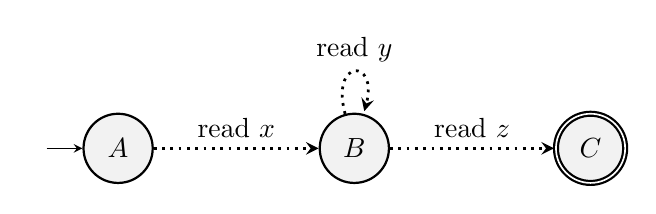
\begin{tikzpicture}
\node[state, initial] (A) {$A$};
\node[state, right of=A] (B) {$B$};
\node[state, accepting, right of=B] (C) {$C$};
\draw (A) edge[mydotted,above] node{read $x$} (B)
(B) edge[mydotted,above] node{read $z$} (C)
(B) edge[mydotted,loop above] node{read $y$} (B);
\end{tikzpicture}
\caption{Illustration of lemma with DFA}
\label{fig:my_label}
\end{figure}


\section{Proof:}
\begin{proof}
Let $D=(Q,\Sigma, \delta, q_0,F)$ be a DFA accepting $L$ and $p$ be the number of states of $D$
Let $w=w_1w_2\cdots w_n\in L$ and  $\mid w\mid =n$ and $n\ge p$.
Let the sequence of states $w$ go through be $r_1,r_2\cdots r_{n+1}$
$$r_{i+1}=\delta(r_i,w_i)\forall i\in [1,n]$$
According to pigeonhole principle($p+1$ pigeons and $p$ pigeonholes) , the first $p+1$ states must have a repetition of a state, let the first occurrence of the state $r_a$ and the occurrence be $r_b$ and also $b\le p+1$. 

Now let $$x=w_1\cdots w_{a-1}$$ $$y=w_a\cdots w_{b-1}$$ $$z=w_b\cdots w_n$$
For $i\ge0$, $w'=xy^iz$ , $x$ takes $D$ from $r_1$ to $r_a$, $y$ takes $D$ from $r_a$ to $r_a$ and $z$ takes $D$ from $r_a$ to $r_n+1$, hence $D$ must accept $w'$ . Furthermore,
$$a\ne b\implies \mid y\mid>0$$
$$b\le p+1\implies b-1\le p \implies \mid xy\mid \le p$$
\end{proof}

\section{Application:}
Pumping lemma can be used to prove that a language is not regular by "Proof by Contradiction". We assume that the language is regular and choose a string whose length is greater than the pumping constant and that can't be pumped and we reach a contradiction by failing to divide the string into any $x,y,z$ and then put forward that the language is not regular.

It is important to note that the converse of pumping lemma is not true i.e. a language that satisfies these conditions is not necessarily a regular language.

\subsection{Example 1}

Prove that the language $L=\{0^n1^n\mid n\in \mathbb{N}\}$ is not regular.

\begin{proof}
Let us assume $L$ to be a regular language. Now according to pumping lemma $\exists(p\ge1)$.
Let the string $w\in L$ and $$w=0^p1^p$$ $$\mid w\mid=2p>p $$ $$w=xyz$$
As $\mid xy\mid\le p$, $xy=0^q$ where $q=\mid xy\mid\le p$. Let $y=0^k$ and $x=0^{q-k}$ where $k\in[1,q]$ and $z=0^{p-q}1^p$.
Now by statement 3 of lemma, 
$$(\forall n\ge0)(xy^nz)\in L$$
$$\implies 0^{q-k}0^{kn}0^{p-q}1^p\in L$$
$$\implies 0^{k(n-1)+p}1^p\in L$$
Since $k\in[1,p]$, $k(n-1)+p\ne p$ hence $0^{k(n-1)+p}1^p\notin L$. A contradiction!

Hence, the initial assumption was wrong and the language $L$ is not regular.
\end{proof}

\subsection{Example 2}

Prove that the language $L=\{ss\mid s\in \{ 0,1\}^*\}$ is not regular.

\begin{proof}
Let us assume $L$ to be a regular language. Now according to pumping lemma $\exists(p\ge1)$.
Let the string $w\in L$ and $$w=0^p10^p1$$ $$\mid w\mid=2p+2>p $$ $$w=xyz$$
As $\mid xy\mid\le p$, $xy=0^q$ where $q=\mid xy\mid\le p$. Let $y=0^k$ and $x=0^{q-k}$ where $k\in[1,q]$ and $z=0^{p-q}10^p1$.
Now by statement 3 of lemma, 
$$(\forall n\ge0)(xy^nz)\in L$$
$$\implies 0^{q-k}0^{kn}0^{p-q}10^p1\in L$$
$$\implies 0^{k(n-1)+p}10^p1\in L$$
Since $k\in[1,p]$, $k(n-1)+p\ne p$ hence $0^{k(n-1)+p}1^p\notin L$. A contradiction!

Hence, the initial assumption was wrong and the language $L$ is not regular.
\end{proof}

\subsection{Example 3}

Prove that the language $L=\{1^{n^2}\mid n\ge 0\}$ is not regular.

\begin{proof}
Let us assume $L$ to be a regular language. Now according to pumping lemma $\exists(p\ge1)$.
Let the string $w\in L$ and $$w=1^{p^2}$$ $$\mid w\mid=p^2>p $$ $$w=xyz$$
As $\mid xy\mid\le p$, $xy=1^q$ where $q=\mid xy\mid\le p$. Let $y=1^k$ and $x=1^{q-k}$ where $k\in[1,q]$ and $z=1^{p^2-q}$.
Now by statement 3 of lemma, for $n=2$
$$(xy^2z)\in L$$
$$\implies 1^{q-k}1^{2k}1^{p^2-q}\in L$$
$$\implies 1^{p^2+k}\in L$$
$p^2+k$ must be a perfect square. $1\le k\le q$ and $q\le p$ implies $1\le k\le p$ 
$$(1\le k\le q)\wedge (q\le p)\implies 1\le k\le p$$
The next perfect square after $p^2$ is $(p+1)^2$,so there are no perfect square in $(p^2,(p+1)^2)$, Also, $(p+1)^2-p^2=2p+1$, But
$$k\le p$$
$$k< 2p$$
$$k< 2p+1$$
So, $1^{p^2+k}\notin L$. A contradiction!

Hence, the initial assumption was wrong and the language $L$ is not regular.
\end{proof}

\subsection{Example 4}

Prove that the language $L=\{0^i1^j\mid i>j\}$ is not regular.

\begin{proof}
Let us assume $L$ to be a regular language. Now according to pumping lemma $\exists(p\ge1)$.
Let the string $w\in L$ and $$w=0^p1^{p-1}$$ $$\mid w\mid=2p-1\ge p $$ $$w=xyz$$
As $\mid xy\mid\le p$, $xy=0^q$ where $q=\mid xy\mid\le p$. Let $y=0^k$ and $x=0^{q-k}$ where $k\in[1,q]$ and $z=0^{p-q}1^{p-1}$.
Now by statement 3 of lemma, for $n=0$
$$(xy^0z)\in L$$
$$\implies 0^{q-k}0^{0}0^{p-q}1^{p-1}\in L$$
$$\implies 0^{p-k}1^{p-1}\in L$$
Since $k\in[1,p]$, $p-k\le p-1$ hence $0^{p-k}1^{p-1}\notin L$. A contradiction!

Hence, the initial assumption was wrong and the language $L$ is not regular.
\end{proof}

\subsection{Example 5}

Prove that the language $L=\{0^n1^n2^n\mid n\ge0\}$ is not regular.

\begin{proof}
Let us assume $L$ to be a regular language. Now according to pumping lemma $\exists(p\ge1)$.
Let the string $w\in L$ and $$w=0^p1^p2^p$$ $$\mid w\mid=3p>p $$ $$w=xyz$$
As $\mid xy\mid\le p$, $xy=0^q$ where $q=\mid xy\mid\le p$. Let $y=0^k$ and $x=0^{q-k}$ where $k\in[1,q]$ and $z=0^{p-q}1^p2^p$.
Now by statement 3 of lemma,
$$(\forall n\ge0)(xy^nz)\in L$$
$$\implies 0^{q-k}0^{kn}0^{p-q}1^p2^p\in L$$
$$\implies 0^{k(n-1)+p}1^p2^p\in L$$
Since $k\in[1,p]$, $k(n-1)+p\ne p$ hence $0^{k(n-1)+p}1^p2^p\notin L$. A contradiction!

Hence, the initial assumption was wrong and the language $L$ is not regular.
\end{proof}

\subsection{Example 6}

Prove that the language $L=\{sss\mid s\in \{ 0,1\}^*\}$ is not regular.

\begin{proof}
Let us assume $L$ to be a regular language. Now according to pumping lemma $\exists(p\ge1)$.
Let the string $w\in L$ and $$w=0^p10^p10^p1$$ $$\mid w\mid=3p+3>p $$ $$w=xyz$$
As $\mid xy\mid\le p$, $xy=0^q$ where $q=\mid xy\mid\le p$. Let $y=0^k$ and $x=0^{q-k}$ where $k\in[1,q]$ and $z=0^{p-q}1^p0^p1$.
Now by statement 3 of lemma, 
$$(\forall n\ge0)(xy^nz)\in L$$
$$\implies 0^{q-k}0^{kn}0^{p-q}10^p10^p1\in L$$
$$\implies 0^{k(n-1)+p}10^p10^p1\in L$$
Since $k\in[1,p]$, $k(n-1)+p\ne p$ hence $0^{k(n-1)+p}10^p10^p1\notin L$. A contradiction!

Hence, the initial assumption was wrong and the language $L$ is not regular.
\end{proof}

\subsection{Example 7}

Prove that the language $L=\{1^{2^n}\mid n\ge 0\}$ is not regular.

\begin{proof}
Let us assume $L$ to be a regular language. Now according to pumping lemma $\exists(p\ge1)$.
Let the string $w\in L$ and $$w=1^{2^p}$$ $$\mid w\mid=2^p>p $$ $$w=xyz$$
As $\mid xy\mid\le p$, $xy=1^q$ where $q=\mid xy\mid\le p$. Let $y=1^k$ and $x=1^{q-k}$ where $k\in[1,q]$ and $z=1^{2^p-q}$.
Now by statement 3 of lemma, for $n=2$
$$(xy^2z)\in L$$
$$\implies 1^{q-k}1^{2k}1^{2^p-q}\in L$$
$$\implies 1^{2^p+k}\in L$$                            

$2^p+k$ must be a power of 2. But, as $k\in[1,p]$

$$2^p>k$$
$$2^p+2^p>k+2^p$$
$$2^{p+1}>2^p+k$$
And no power of 2 lies in $(2^p,2^{p+1})$. So, $1^{2^p+k}\notin L$. A contradiction!

Hence, the initial assumption was wrong and the language $L$ is not regular.
\end{proof}

\begin{thebibliography}{9}
\bibitem{sipser}

Michael Sipser,
\textit{Introduction to the Theory of Computation},
Cengage Learning, 2012.

\bibitem{enwiki:1264121825}
Wikipedia contributors,
\textit{Pumping lemma for regular languages --- Wikipedia, The Free Encyclopedia},
2024,
\url{https://en.wikipedia.org/w/index.php?title=Pumping_lemma_for_regular_languages&oldid=1264121825},

\bibitem{stanford}
Stanford University,
\textit{CS103: Mathematical Foundations of Computing},
\url{https://web.stanford.edu/class/cs103/}

\end{thebibliography}

\end{document}

